\documentclass{article}
\usepackage{titletoc}
\usepackage{lipsum}
\usepackage{graphicx}
\usepackage[a4, portrait, margin=1.45in]{geometry}
\usepackage[utf8]{inputenc}
\usepackage{listings}
\usepackage{xcolor}

\definecolor{codegreen}{rgb}{0,0.6,0}
\definecolor{codegray}{rgb}{0.5,0.5,0.5}
\definecolor{codepurple}{rgb}{0.58,0,0.82}
\definecolor{backcolour}{rgb}{0.95,0.95,0.92}

\lstdefinestyle{mystyle}{
    backgroundcolor=\color{backcolour},   
    commentstyle=\color{codegreen},
    keywordstyle=\color{magenta},
    numberstyle=\tiny\color{codegray},
    stringstyle=\color{codepurple},
    basicstyle=\ttfamily\footnotesize,
    breakatwhitespace=false,         
    breaklines=true,                 
    captionpos=b,                    
    keepspaces=true,                 
    numbers=left,                    
    numbersep=5pt,                  
    showspaces=false,                
    showstringspaces=false,
    showtabs=false,                  
    tabsize=2
}

\lstset{style=mystyle}
\usepackage{titling}
\renewcommand\maketitlehooka{\null\mbox{}\vfill}
\renewcommand\maketitlehookd{\vfill\null}
\newcommand{\subtitle}[1]{%
  \posttitle{%
    \par\end{center}
    \begin{center}\large#1\end{center}
    \vskip0.5em}%
}
\title{\textbf{Gestionarea unui magazin de muzica}}
\subtitle{\textbf{Proiect SGBD}}
\author{Ciaușu Nicoleta \\ Grupa 234}
\date{}

\begin{document}
\begin{titlingpage}
\maketitle
\end{titlingpage}
\newpage
% The complete ToC 
\renewcommand{\contentsname}{Cuprins}
\tableofcontents

\clearpage

% ToC of the main sections

\section{Introducere}
Am ales sa modelez o baza de date a unui magazin online de muzica. Scopul acestei baze de date este de a inventaria albumele, piesele, genurile muzicale disponibile pe site si de a tine o evidenta a comenzilor facute de clienti.

Baza de date cuprinde:
\begin{enumerate}
    \item Lista clientilor
    \item Lista comenzilor efectuate de clienti
    \item Lista albumelor din magazin
    \item Lista genurilor muzicale disponibile in magazin
    \item Lista pieselor
    \item Lista artistilor
    \item Pastrarea detaliilor comenzilor (ce albume a comandat fiecare client)
    \item Lista caselor de discuri ale caror albume sunt prezente in magazin
\end{enumerate}

\newpage

\section{Diagrama E/R}
Diagrama Entitate-Relatie a bazei de date este urmatoarea:

\vspace{0.5cm}

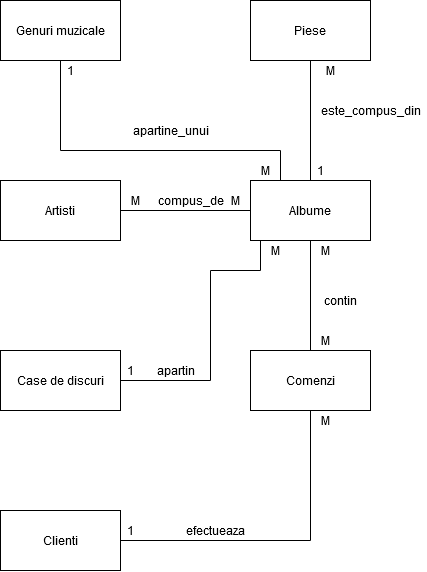
\includegraphics[width=0.9\textwidth]{2-erd-22.png}

\newpage
\section{Diagrama Conceptuala}
Dupa ce am creat diagrama E/R, am construit diagrama conceptuala, care evidentiaza tabelele asociative, cat si listeaza coloanei fiecarui tabel din baza de date.


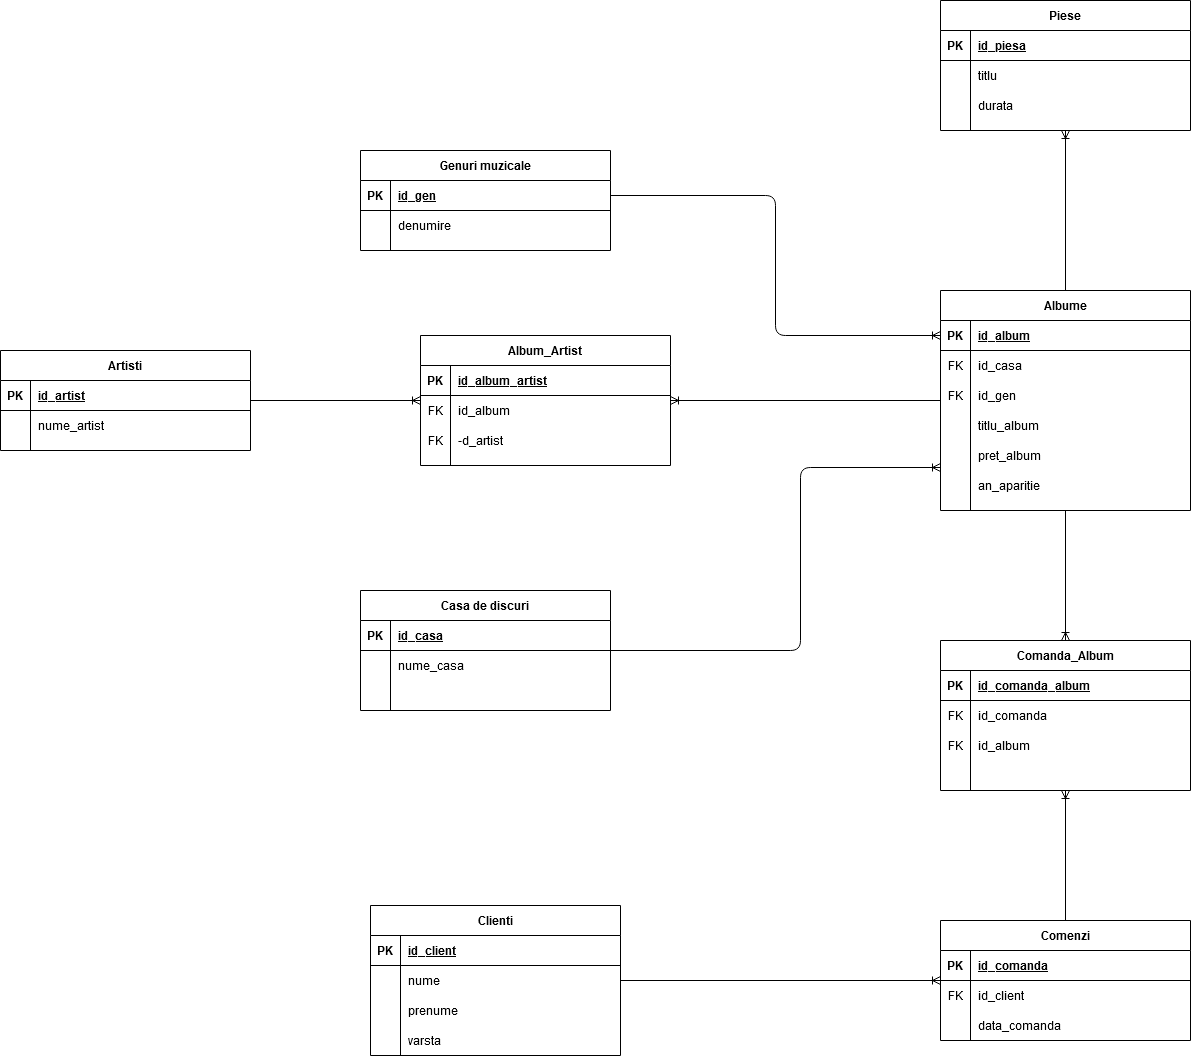
\includegraphics[width=\textwidth]{3-diag.png}

\newpage

\section{Crearea Bazei de Date}
Mai intai am creat toate tabelele care nu contin chei straine. Acestea sunt: Clienti, Piese, Genuri, CaseDiscuri, Artisti.

\begin{lstlisting}[language=SQL, title=Crearea tabelelor fara chei straine]
Create table Clienti(
	id_client number(7) primary key,
	nume varchar(50),
	prenume varchar(50),
	varsta number(7)); 

create table Piese(
    id_piesa number(7) primary key,
    titlu_piesa varchar(50),
    durata_piesa number(7));
    
create table Genuri(
    id_gen number(7) primary key,
    nume_gen varchar(50),
    constraint nume_unic unique (nume_gen));
    
create table Case_Discuri(
    id_casa number(7) primary key,
    nume_casa varchar(50));

create table Artisti(
    id_artist number(7) primary key,
    nume_artist varchar(50));

\end{lstlisting}

Dupa aceea, am creat tabelele care au in componenta lor chei straine, adaugand totodata si constrangerile.

\begin{lstlisting}[language=SQL, title=Crearea tabelelor cu chei straine si tabelele asociative]
create table Comenzi(
    id_comanda number(7) primary key,
    id_client number(7),
    constraint FK_ComandaClient foreign key (id_client)
    references Clienti(id_client),
    data_comanda DATE);
        
create table Albume(
    id_album number(7) primary key,
    id_casa number(7),
    id_gen number(7),
    constraint FK_CasaAlbum foreign key (id_casa)
    references Case_Discuri(id_casa),
    constraint FK_GenAlbum foreign key (id_gen)
    references Genuri(id_gen),
    titlu_album varchar(50),
    pret_album number(7),
    an_aparitie number(7));

create table Album_Artist(
    id_album_artist number(7) primary key,
    id_album number(7),
    id_artist number(7),
    constraint FK_AlbumArtist foreign key (id_album)
    references Albume(id_album),
    constraint FK_AlbumArtist2 foreign key (id_artist)
    references Artisti(id_artist));

create table Comanda_Album(
    id_comanda_album number(7) primary key,
    id_comanda number(7),
    id_album number(7),
    constraint FK_ComandaAlbum foreign key (id_comanda)
    references Comenzi(id_comanda),
    constraint FK_ComandaAlbum2 foreign key (id_album)
    references Albume(id_album));
\end{lstlisting}

\newpage
\section{Popularea bazei de date}

Dupa aceea, a venit momentul in care a trebuit sa populez baza de date. Cum nu mi-am dorit sa o umplu de date incoerente, nici sa scriu de mana query-urile de insert, am folosit ceea ce am invatat la Programarea Algoritmilor in semestrul 1 si am scris in Python un script care mi-a generat query-urile pentru popularea bazei mele de date.

Pentru fiecare entitate (Client, Gen, Album etc...) am definit niste fisiere text in care am pus cuvintele pe care am dorit sa le folosesc:
\begin{enumerate}
    \item Pentru numele clientilor am generat toate numele posibile din 7 nume si 7 prenume
    \item Pentru genuri am ales cele mai comune 7 genuri muzicale de pe Billboard top 100
    \item Pentru artisti am ales cativa dintre cei mai populari artisti din toate timpurile
    \item Pentru numele albumelor am folosit un generator de nume de albume
    \item Pentru numele pieselor, am generat nume folosind o lista de cuvinte
\end{enumerate}

Asadar, am scris urmatorul script in Python care rulat imi genereaza datele tabelelor, atat ale entitatilor cat si ale tabelelor asociative (pentru asta am retinut id-urile in vectori si am facut asocieri aleatoriu):

\begin{lstlisting}[language=Python, title=Generarea datelor folosind Python]
# generez inserturile cu care voi popula baza de date

from pathlib import Path
import random
import time
import datetime
#### Clienti ####
nume = Path("nume.txt").read_text().split('\n');
prenume = Path("prenume.txt").read_text().split('\n');

clienti = []
piese = []
genuri = []
artisti = []
case_discuri = []
albume = []
index = 1;
for n in nume:
    for p in prenume:
        index+=1
        clienti.append([index,n,p,random.randint(16,40)])



### Piese ###
# generez titlu (1-3 cuvinte) si durata
d_piese = Path("piese.txt").read_text().split('\n');


numar_piese = 200
while numar_piese > 0:
    numar_piese-=1;
    numar_cuvinte=random.randint(1,4);
    titlu = ""
    while numar_cuvinte > 0:
        titlu += random.choice(d_piese) + " ";
        numar_cuvinte-=1;
    titlu.strip();
    index+=1
    numar_piese-=1
    piese.append([index,titlu,random.randint(2,6)])

### Genuri muzicale ###

d_genuri = Path("genuri.txt").read_text().split('\n');
for g in d_genuri:
    index+=1
    genuri.append([index, g]);
    
### Case de discuri ###

d_case =Path("case_discuri.txt").read_text().split('\n'); 
for c in d_case:
    index+=1
    case_discuri.append([index, c]);

### Artisti ###

d_artisti = Path("artisti.txt").read_text().split('\n');
for a in d_artisti:
    index+=1
    artisti.append([index, a]);

### Albume ###

d_albume = Path("albume.txt").read_text().split('\n');
for a in d_albume:
    index+=1
    #id, id_casa, id_gen, nume, pret, an
    albume.append([index,random.choice(case_discuri)[0],random.choice(genuri)[0], a, random.randint(10,100), random.randint(1965,2019)]);

### Comenzi ###
nr_comenzi = 50
comenzi = []
while nr_comenzi>0:
    index+=1
    now = datetime.datetime.now()
    comenzi.append([index,random.choice(clienti)[0],now.strftime('%Y-%m-%d %H:%M:%S')])

    nr_comenzi-=1



### Album_Artist ###
# un album poate fi compus de 1-3 artisti
album_artist = []
for album in albume:
    nr_albume = random.randint(1,3);
    while nr_albume > 0:
        index+=1
        album_artist.append([index,album[0],random.choice(artisti)[0]])
        nr_albume-=1

## Comanda_Album ###
# o comanda poate contine mai multe albume
# id_album_comanda, id_comanda, id_album
comanda_album = []
for comanda in comenzi:
    # o comanda poate avea intre 1 si 5 albume
    nr_albume = random.randint(1,5)
    while nr_albume > 0:
        index+=1
        comanda_album.append([index,comanda[0],random.choice(albume)[0]])
        nr_albume-=1


open('script_generare.sql', 'w').close()
with open("script_generare.sql",'a') as output:
    output.write(Path("creare_tabele.txt").read_text())
    for c in clienti:
        output.write("INSERT INTO Clienti (id_client, nume, prenume, varsta) VALUES ({0}, '{1}', '{2}', {3});\n".format(c[0],c[1],c[2],c[3]));
    for p in piese:
        output.write("INSERT INTO Piese (id_piesa, titlu_piesa, durata_piesa) VALUES ({0}, '{1}', {2});\n".format(p[0],p[1],p[2]));
    for g in genuri:
        output.write("INSERT INTO Genuri (id_gen, nume_gen) VALUES ({0}, '{1}');\n".format(g[0],g[1]));
    for c in case_discuri:
        output.write("INSERT INTO Case_Discuri (id_casa, nume_casa) VALUES ({0}, '{1}');\n".format(c[0],c[1]));
    for a in artisti:
        output.write("INSERT INTO Artisti (id_artist, nume_artist) VALUES ({0}, '{1}');\n".format(a[0],a[1]));
    for c in comenzi:
        output.write("INSERT INTO Comenzi (id_comanda, id_client, data_comanda) VALUES ({0}, {1}, TO_DATE('{2}','yyyy-mm-dd hh24:mi:ss'));\n".format(c[0],c[1],c[2]));
    for a in albume:
        output.write("INSERT INTO Albume (id_album, id_casa, id_gen, titlu_album, pret_album, an_aparitie) VALUES ({0}, {1}, {2}, '{3}', {4}, {5});\n".format(a[0],a[1],a[2],a[3],a[4],a[5]))
    for aa in album_artist:
        output.write("INSERT INTO Album_Artist (id_album_artist, id_album, id_artist) VALUES ({0}, {1}, {2});\n".format(aa[0],aa[1],aa[2]))
    for ca in comanda_album:
        output.write("INSERT INTO Comanda_Album (id_comanda_album, id_comanda, id_album) VALUES ({0}, {1}, {2});\n".format(ca[0],ca[1],ca[2]))
print("Am generat in fiserul script_generare.sql query-urile necesare.")
\end{lstlisting}

Tot ce a mai ramas de facut a fost sa rulez acest script generat de mine in SQL Developer. Generarea a avut loc cu succes.

\vspace{0.5cm}

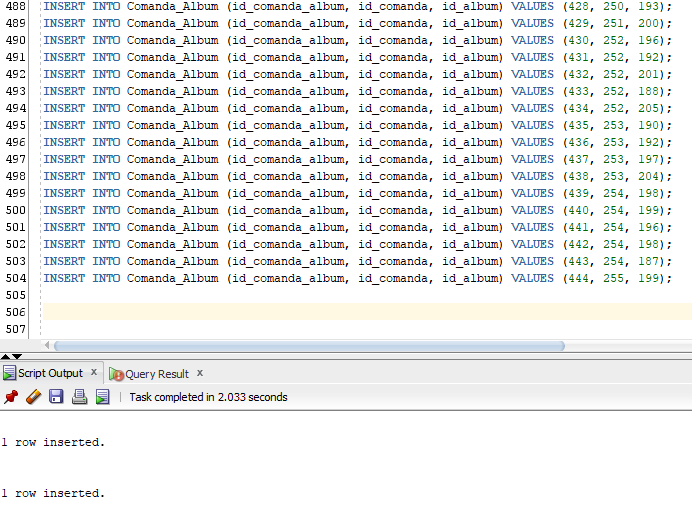
\includegraphics[width=\textwidth]{4-gen.png}

\newpage
\section{Cerinta 6}
Pentru cerinta 6, am implementat o procedura care determina si afiseaza date despre comanda cu valoarea maxima (ce valoare are, data la care a fost efectuata, respectiv ce albume contine). Daca exista mai multe comenzi cu aceeasi valoare maxima, se vor afisa toate. Pentru compunerea raspunsului(retinerea albumelor) am folosit un tablou imbricat.

\begin{lstlisting}[language=SQL, title=Cerinta 6]
--6 - tablouri
set serveroutput on;

select id_comanda,a.pret_album from comanda_album ca join albume a on ca.id_album = a.id_album;

create or replace procedure AflaComandaMaxima 
is
    type tbl2 is table of number; --tablou imbricat (numerotare crescatoare)
    res tbl2:=tbl2();
    max_sum number;
    
    comanda comenzi%rowtype;
begin
    -- fac sume pe comenzile clientilor
    select max(sum(a.pret_album)) 
    into max_sum
    from comanda_album ca join albume a on ca.id_album = a.id_album
    group by id_comanda;
     
    select id_comanda
    bulk collect into res
    from comanda_album ca join albume a on ca.id_album = a.id_album
    group by id_comanda
    having sum(pret_album) = max_sum;
     
    for i in res.first .. res.last loop
        select *
         into comanda
         from comenzi
        where id_comanda = res(i);
        dbms_output.put_line('Comanda cu numarul ' || comanda.id_comanda || ' efectuata la data: ' || comanda.data_comanda || ' are valoarea ' || max_sum || ' lei si contine albumele: ');
        
        for j in (select * 
         from albume a join comanda_album ca
         on a.id_album = ca.id_album
         where ca.id_comanda = res(i)) loop
            dbms_output.put_line(j.titlu_album || ' ' || j.pret_album);
         end loop;
    end loop;
end;
/
\end{lstlisting}

\vspace{0.5cm}

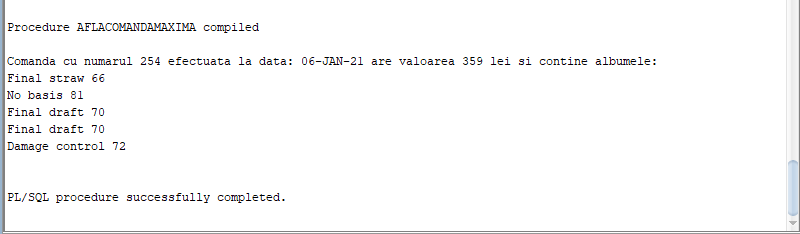
\includegraphics[width=\textwidth]{6.png}

\newpage
\section{Cerinta 7}
Magazinul doreste sa efectueze periodic o statistica a genurilor muzicale, respectiv a numarului de albume de acel gen disponibil, pentru a determina ce albume sa mai aduca astfel incat sa aiba un portofoliu cat mai divers si sa fie cat mai atractiv pentru clienti. Pentru a indeplini acest lucru, am creat procedura StatisticaGenuri, care imi afiseaza fiecare gen si numarul de albume de acel gen.

\vspace{0.5cm}
\begin{lstlisting}[language=SQL, title=Cerinta 7]
--7 - cursor explicit

create or replace procedure StatisticaGenuri
is
    v_nr number(7);
    v_nume_gen genuri.nume_gen%TYPE;
    CURSOR c is
        select nume_gen, count(id_album)
        from albume ag join genuri g on ag.id_gen = g.id_gen
        group by nume_gen;
begin
    open c;
    loop
        fetch c into v_nume_gen, v_nr;
        exit when c%notfound;
        if v_nr=0 then
            dbms_output.put_line('Genul muzical ' || v_nume_gen || ' nu are niciun album disponibil');
        elsif v_nr=1 then
            dbms_output.put_line('Genul muzical ' || v_nume_gen || ' are un album disponibil');
        else
            dbms_output.put_line('Genul muzical ' || v_nume_gen || ' are ' || v_nr || ' albume disponibile');
        end if;
    end loop;
    close c;
end;
/

execute statisticagenuri;
/
\end{lstlisting}

\vspace{0.5cm}

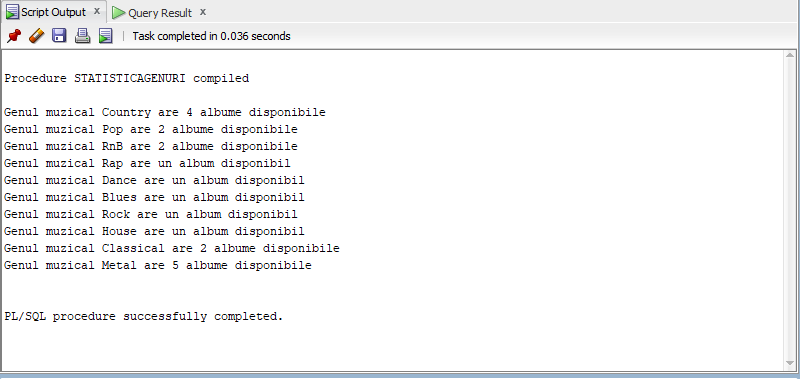
\includegraphics[width=\textwidth]{7.png}

\newpage
\section{Cerinta 8}
Administratorii site-ului vor sa stie pentru o suma data V, care sunt clientii care au efectuat comenzi cu valoare mai mare sau egala cu V, si cate comenzi de acest fel au efectuat.

Am folosit tabelele Clienti, Comenzi, ComandaAlbum, Albume.


\begin{lstlisting}[language=SQL, title=Cerinta 8]
create or replace procedure VeziClientiComenziMaiMariCa(valoare number)
is
        type tbl is table of number index by binary_integer;
        numar_comenzi tbl;
        v_id_client number(7);
        v_id_comanda number(7);
        v_suma number(7);
        cursor c is
            select c.id_client,co.id_comanda, sum(a.pret_album) "Valoare comanda"
            from clienti c 
            join comenzi co on c.id_client = co.id_client
            join comanda_album ca on co.id_comanda = ca.id_comanda
            join albume a on ca.id_album = a.id_album
            group by co.id_comanda, c.id_client
	    having sum(a.pret_album) >= valoare;
        
        v_client clienti%rowtype;
        ok number(1):=0;
        valoare_invalida exception;
begin
    if (valoare <= 0) then
        raise valoare_invalida;
    end if;
    --initializare
    for cc in (select id_client from clienti) loop
        numar_comenzi(cc.id_client):=0;
    end loop;
    
    open c;
    loop
        fetch c into v_id_client, v_id_comanda, v_suma;
        exit when c%notfound;
        numar_comenzi(v_id_client):= numar_comenzi(v_id_client) + 1;
    end loop;
    
       for i in numar_comenzi.first .. numar_comenzi.last loop
            if(numar_comenzi.exists(i)) then
                select *
                into v_client
                from clienti
                where id_client = i;
                if(numar_comenzi(i) > 0) then
                    ok:=1;
                    if (numar_comenzi(i) = 1) then
                        dbms_output.put_line('Clientul ' || v_client.prenume || ' ' || v_client.nume || ' a plasat o comanda cu valoare > '|| valoare ||' lei');
                    else
                        dbms_output.put_line('Clientul ' || v_client.prenume || ' ' || v_client.nume || ' a plasat ' || numar_comenzi(i) ||' comenzi cu valoare >  '|| valoare ||' lei');
                    end if;        
                end if;
            end if;
        end loop;
        
        if ok=0 then
            dbms_output.put_line('Nu exista comenzi mai mari decat aceasta valoare.');
        end if;
        -- nu putem avea "too many rows" pentru ca numaram liniile intr-un vector si afisam doar nr de linii
    exception
        when valoare_invalida then
            dbms_output.put_line('Ai cerut o valoare negativa.');
        when others then
         dbms_output.put_line('Alta eroare in VeziClientiComenziMaiMariCa');

end;
/

execute veziclienticomenzimaimarica(200);

execute veziclienticomenzimaimarica(-50); --exceptie: valoare invalida
\end{lstlisting}

\vspace{0.5cm}

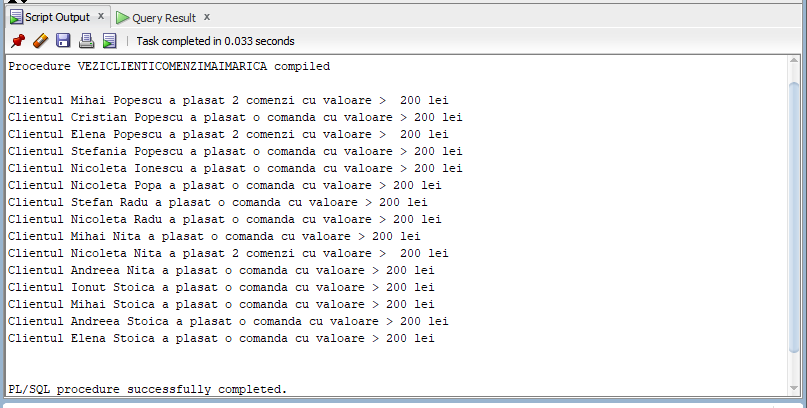
\includegraphics[width=\textwidth]{8.png}

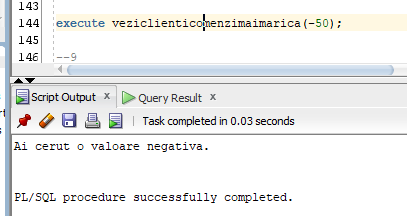
\includegraphics[width=\textwidth]{aaa.png}

\newpage
\section{Cerinta 9}
Pentru crearea unor oferte promotionale personalizate, administratorii isi doresc sa afle care este genul muzical preferat al fiecarui client. Pentru aceasta functionalitate am creat procedura GenMuzicalFavorit, care afiseaza o lista cu toti clientii si genul lor muzical favorit. Daca nu au un gen preferat (au 2 genuri cu numarul maxim de albume cumparate), sau nu au efectuat nicio comanda, se va afisa si acest lucru.

Am folosit tabelele Clienti, Comenzi, ComandaAlbum, Albume, Genuri.

\begin{lstlisting}[language=SQL, title=Cerinta 9]

--9
-- afla genul muzical preferat al fiecarui client
set serveroutput on;
create or replace procedure GenMuzicalFavorit
is
    type ob_array is record(
        nume_gen genuri.nume_gen%type,
        nr_piese number(7),
        nume_client clienti.nume%type,
        prenume_client clienti.prenume%type
    );
    type tbl is table of ob_array index by binary_integer;
    rezultate tbl;
    tmp ob_array;
    cursor c is
        select c.id_client, c.nume, c.prenume, g.nume_gen, count(g.nume_gen)
        from clienti c 
        left join comenzi co on c.id_client = co.id_client
        left join comanda_album ca on co.id_comanda = ca.id_comanda
        left join albume a on ca.id_album = a.id_album
        left join genuri g on g.id_gen = a.id_gen
        group by c.id_client, c.nume, c.prenume, g.nume_gen
        order by id_client, count(g.nume_gen) desc;
        
    v_id_client clienti.id_client%type;
    v_nume_gen genuri.nume_gen%type;
    v_nr_piese number(7);
    v_nume_client clienti.nume%type;
    v_prenume_client clienti.prenume%type;
begin
    --initializare
    tmp.nr_piese:=0;
    for c in (select id_client from clienti) loop
        rezultate(c.id_client):=tmp;
    end loop;

    open c;
    loop
        fetch c into v_id_client, v_nume_client, v_prenume_client, v_nume_gen, v_nr_piese;
        if(rezultate(v_id_client).nr_piese = 0) then
            rezultate(v_id_client).nume_gen := v_nume_gen;
            rezultate(v_id_client).nume_client := v_nume_client;
            rezultate(v_id_client).prenume_client := v_prenume_client;

            rezultate(v_id_client).nr_piese := v_nr_piese;
        elsif(rezultate(v_id_client).nr_piese = v_nr_piese) then
            rezultate(v_id_client).nr_piese := -1;
        end if;
        exit when c%notfound;
    end loop;
    
    for i in rezultate.first .. rezultate.last loop
        if rezultate.exists(i) then
            if (rezultate(i).nr_piese = -1) then
                dbms_output.put_line(rezultate(i).nume_client ||' '||  rezultate(i).prenume_client ||' nu are un gen preferat');
            elsif (rezultate(i).nr_piese = 0) then
                dbms_output.put_line(rezultate(i).nume_client ||' '||  rezultate(i).prenume_client ||' nu a efectuat nicio comanda pana acum');
            else
                dbms_output.put_line(rezultate(i).nume_client ||' '||  rezultate(i).prenume_client ||' are genul preferat ' || rezultate(i).nume_gen ||', cu '|| rezultate(i).nr_piese||' albume comandate de acest gen');
            end if;
        end if;
    end loop;
    
exception
    when others then
         dbms_output.put_line('Alta eroare in GenMuzicalFavorit');
end;
/

execute genmuzicalfavorit;
\end{lstlisting}
\vspace{0.5cm}

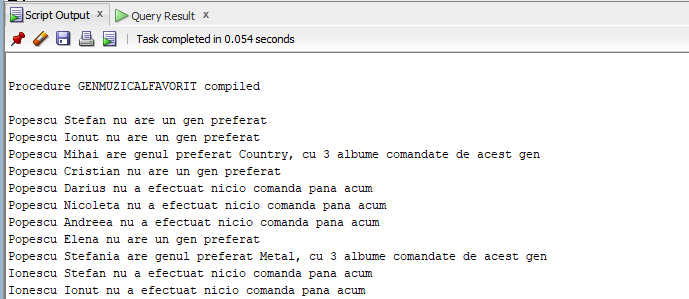
\includegraphics[width=\textwidth]{9.png}

\newpage
\section{Cerinta 10}
Data de 1 a fiecarei luni este momentul cand se primesc noile albume digitale. Asadar, administratorii au decis sa permita manipularea tabelului Albume doar atunci, pentru a incerca sa minimizeze accidentele.

\begin{lstlisting}[language=SQL, title=Cerinta 10]
-- 10
-- trigger lmd instructiune
-- trigger care sa permita lucrul asupra tabelului de albume doar pe data de 1 a fiecarei luna
-- (atunci se primesc albumele noi)

create or replace trigger trig1
    before insert or update or delete on albume
begin
    if (to_char(sysdate,'D') != 1) then
    	raise_application_error(-20001,'Nu se pot modifica albumele decat pe data de 1!');
    end if;
end;
/
--test
INSERT INTO Albume (id_album, id_casa, id_gen, titlu_album, pret_album, an_aparitie) VALUES (22222, 169, 162, 'Damage control', 61, 1979);
\end{lstlisting}

\vspace{0.5cm}

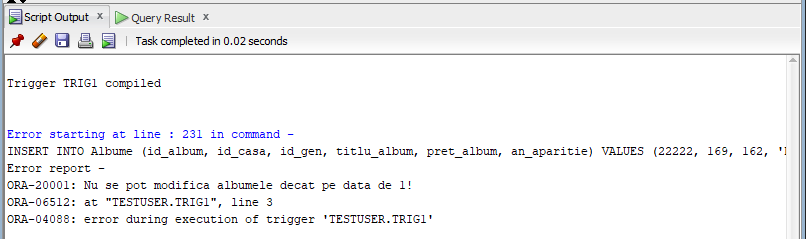
\includegraphics[width=\textwidth]{10.png}

\newpage
\section{Cerinta 11}
Pentru a preveni erorile umane, administratorii au decis ca la introducerea unui client nou sa se faca o verificare care sa se asigure ca numele si prenumele clientului nu poate avea decat litere.


\begin{lstlisting}[language=SQL, title=Cerinta 11]
--11
-- trigger lmd linie
-- nume doar cu litera mica si mare
create or replace function AreDoarLitere
    (nume clienti.nume%type)
return boolean is 
	rasp boolean:=false;
begin
    if (LENGTH(TRIM(TRANSLATE(nume, 'abcdefghijklmnopqrstuvwxyzABCDEFGHIJKLMNOPQRSTUVWXYZ', ' '))) is null) then
        rasp:=true;
    end if;
    return rasp;
end AreDoarLitere;
/
create or replace trigger trig2
    before insert or update of nume, prenume on clienti
    for each row
    begin
    if (AreDoarLitere(:NEW.nume) = false) then
        RAISE_APPLICATION_ERROR(-20002,'Numele poate avea doar litere.');
    end if;
    end;
/
INSERT INTO Clienti (id_client, nume, prenume, varsta) VALUES (9999, 'Ion@@escu', 'Mihai', 16);
\end{lstlisting}

\vspace{0.5cm}

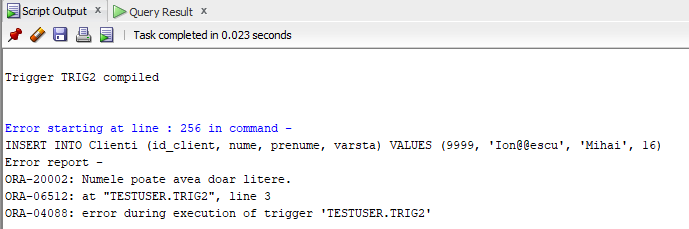
\includegraphics[width=\textwidth]{11.png}

\newpage
\section{Cerinta 12}
Am creat un tabel in care sa pot loga actiunile de LDD din baza mea de date.
Voi retine numele utilizatorului, evenimentul, pe ce tabel a avut loc, si data actiunii.

 \begin{lstlisting}[language=SQL]
create table audit_magazin
(
    utilizator varchar2(30),
    eveniment varchar2(50),
    nume_obiect varchar2(30),
    data date);
 \end{lstlisting}

In continuare, voi defini un trigger care sa imi noteze in acest tabel de fiecare data cand are loc o astfel de actiune.

\begin{lstlisting}[language=SQL, title=Cerinta 12]
--12
-- trigger ldd
-- audit

create or replace trigger actiune_importanta
    after create or drop or alter on schema
begin
    insert into audit_magazin
    values (sys.login_user, sys.sysevent, sys.dictionary_obj_name, sysdate);
end;
/

create table test_trig(id_test number(2) primary key);
drop table test_trig;
select * from audit_magazin;
\end{lstlisting}

\vspace{0.5cm}

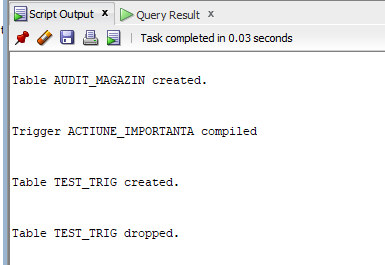
\includegraphics[width=\textwidth]{12-4.png}
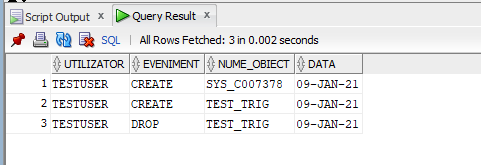
\includegraphics[width=\textwidth]{12-3.png}

\newpage
\section{Cerinta 13}

 \begin{lstlisting}[language=SQL, title=Cerinta 13]
 --pachet

create or replace package pachet_magazin
is
    type ob_array is record(
        nume_gen genuri.nume_gen%type,
        nr_piese number(7),
        nume_client clienti.nume%type,
        prenume_client clienti.prenume%type
    );
    type tbl_ob is table of ob_array index by binary_integer;
    type tbl is table of number index by binary_integer;
    type tbl2 is table of number;
    
    function AreDoarLitere
        (nume clienti.nume%type) return boolean;

    CURSOR c1 is
        select nume_gen, count(id_album)
        from albume ag join genuri g on ag.id_gen = g.id_gen
        group by nume_gen;
        
    cursor c3 is
        select c.id_client, c.nume, c.prenume, g.nume_gen, count(g.nume_gen)
        from clienti c 
        left join comenzi co on c.id_client = co.id_client
        left join comanda_album ca on co.id_comanda = ca.id_comanda
        left join albume a on ca.id_album = a.id_album
        left join genuri g on g.id_gen = a.id_gen
        group by c.id_client, c.nume, c.prenume, g.nume_gen
        order by id_client, count(g.nume_gen) desc;
        
     procedure AflaComandaMaxima;
     procedure StatisticaGenuri;
     procedure VeziClientiComenziMaiMariCa(valoare number);
     procedure GenMuzicalFavorit; 
end pachet_magazin;
/
create or replace package body pachet_magazin
is
    function AreDoarLitere
    (nume clienti.nume%type)
    return boolean is 
        rasp boolean:=false;
    begin
        if (LENGTH(TRIM(TRANSLATE(nume, 'abcdefghijklmnopqrstuvwxyzABCDEFGHIJKLMNOPQRSTUVWXYZ', ' '))) is null) then
            rasp:=true;
        end if;
        return rasp;
    end AreDoarLitere;
    
    procedure StatisticaGenuri
    is
        v_nr number(7);
        v_nume_gen genuri.nume_gen%TYPE;
    begin
        open c1;
        loop
            fetch c1 into v_nume_gen, v_nr;
            exit when c1%notfound;
            if v_nr=0 then
                dbms_output.put_line('Genul muzical ' || v_nume_gen || ' nu are niciun album disponibil');
            elsif v_nr=1 then
                dbms_output.put_line('Genul muzical ' || v_nume_gen || ' are un album disponibil');
            else
                dbms_output.put_line('Genul muzical ' || v_nume_gen || ' are ' || v_nr || ' albume disponibile');
            end if;
        end loop;
        close c1;
    end StatisticaGenuri;
    
    procedure VeziClientiComenziMaiMariCa(valoare number)
    is
            numar_comenzi tbl;
            v_id_client number(7);
            v_id_comanda number(7);
            v_suma number(7);
            cursor c2 is
                select c.id_client,co.id_comanda, sum(a.pret_album) "Valoare comanda"
                from clienti c 
                join comenzi co on c.id_client = co.id_client
                join comanda_album ca on co.id_comanda = ca.id_comanda
                join albume a on ca.id_album = a.id_album
                group by co.id_comanda, c.id_client
            having sum(a.pret_album) >= valoare;  
            v_client clienti%rowtype;
            ok number(1):=0;
            valoare_invalida exception;
    begin
        if (valoare <= 0) then
            raise valoare_invalida;
        end if;
        --initializare
        for cc in (select id_client from clienti) loop
            numar_comenzi(cc.id_client):=0;
        end loop;
        
        open c2;
        loop
            fetch c2 into v_id_client, v_id_comanda, v_suma;
            exit when c2%notfound;
            numar_comenzi(v_id_client):= numar_comenzi(v_id_client) + 1;
        end loop;
        
           for i in numar_comenzi.first .. numar_comenzi.last loop
                if(numar_comenzi.exists(i)) then
                    select *
                    into v_client
                    from clienti
                    where id_client = i;
                    if(numar_comenzi(i) > 0) then
                        ok:=1;
                        if (numar_comenzi(i) = 1) then
                            dbms_output.put_line('Clientul ' || v_client.prenume || ' ' || v_client.nume || ' a plasat o comanda cu valoare > '|| valoare ||' lei');
                        else
                            dbms_output.put_line('Clientul ' || v_client.prenume || ' ' || v_client.nume || ' a plasat ' || numar_comenzi(i) ||' comenzi cu valoare >  '|| valoare ||' lei');
                        end if;        
                    end if;
                end if;
            end loop;
            
            if ok=0 then
                dbms_output.put_line('Nu exista comenzi mai mari decat aceasta valoare.');
            end if;
            -- nu putem avea "too many rows" pentru ca numaram liniile intr-un vector si afisam doar nr de linii
        exception
            when valoare_invalida then
                dbms_output.put_line('Ai cerut o valoare negativa.');
            when others then
             dbms_output.put_line('Alta eroare in VeziClientiComenziMaiMariCa');
    
    end VeziClientiComenziMaiMariCa;
    
    procedure AflaComandaMaxima 
    is
        res tbl2:=tbl2();
        max_sum number;
        
        comanda comenzi%rowtype;
    begin
        -- fac sume pe comenzile clientilor
        select max(sum(a.pret_album)) 
        into max_sum
        from comanda_album ca join albume a on ca.id_album = a.id_album
        group by id_comanda;
         
        select id_comanda
        bulk collect into res
        from comanda_album ca join albume a on ca.id_album = a.id_album
        group by id_comanda
        having sum(pret_album) = max_sum;
         
        for i in res.first .. res.last loop
            select *
             into comanda
             from comenzi
            where id_comanda = res(i);
            dbms_output.put_line('Comanda cu numarul ' || comanda.id_comanda || ' efectuata la data: ' || comanda.data_comanda || ' are valoarea ' || max_sum || ' lei si contine albumele: ');
            
            for j in (select * 
             from albume a join comanda_album ca
             on a.id_album = ca.id_album
             where ca.id_comanda = res(i)) loop
                dbms_output.put_line(j.titlu_album || ' ' || j.pret_album);
             end loop;
        end loop;
    end AflaComandaMaxima;


   procedure GenMuzicalFavorit
    is
        rezultate tbl_ob;
        tmp ob_array;
        v_id_client clienti.id_client%type;
        v_nume_gen genuri.nume_gen%type;
        v_nr_piese number(7);
        v_nume_client clienti.nume%type;
        v_prenume_client clienti.prenume%type;
    begin
        --initializare
        tmp.nr_piese:=0;
        for c in (select id_client from clienti) loop
            rezultate(c.id_client):=tmp;
        end loop;
    
        open c3;
        loop
            fetch c3 into v_id_client, v_nume_client, v_prenume_client, v_nume_gen, v_nr_piese;
            if(rezultate(v_id_client).nr_piese = 0) then
                rezultate(v_id_client).nume_gen := v_nume_gen;
                rezultate(v_id_client).nume_client := v_nume_client;
                rezultate(v_id_client).prenume_client := v_prenume_client;
    
                rezultate(v_id_client).nr_piese := v_nr_piese;
            elsif(rezultate(v_id_client).nr_piese = v_nr_piese) then
                rezultate(v_id_client).nr_piese := -1;
            end if;
            exit when c3%notfound;
        end loop;
        
        for i in rezultate.first .. rezultate.last loop
            if rezultate.exists(i) then
                if (rezultate(i).nr_piese = -1) then
                    dbms_output.put_line(rezultate(i).nume_client ||' '||  rezultate(i).prenume_client ||' nu are un gen preferat');
                elsif (rezultate(i).nr_piese = 0) then
                    dbms_output.put_line(rezultate(i).nume_client ||' '||  rezultate(i).prenume_client ||' nu a efectuat nicio comanda pana acum');
                else
                    dbms_output.put_line(rezultate(i).nume_client ||' '||  rezultate(i).prenume_client ||' are genul preferat ' || rezultate(i).nume_gen ||', cu '|| rezultate(i).nr_piese||' albume comandate de acest gen');
                end if;
            end if;
        end loop;
        
    exception
        when others then
             dbms_output.put_line('Alta eroare in GenMuzicalFavorit');
    end GenMuzicalFavorit;
end pachet_magazin;

 \end{lstlisting}

% \vspace{0.5cm}

% 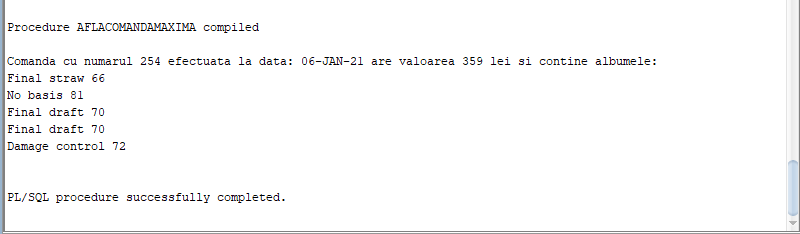
\includegraphics[width=\textwidth]{6.png}


\newpage
\section{Concluzii}
Consider ca acest proiect a reprezentat o ocazie foarte buna de a-mi exersa competentele in materie de sisteme de gestiune a bazelor de date. In plus, in mod particular a fost interesant sa scriu si sa populez o baza de date folosind query-uri create cu un generator scris de mine. Am folosit notiuni precum proceduri, o functie, am folosit tablouri indexate si imbricate, record, cursor.
Cred ca experienta acumulata in urma scrierii acestui proiect ma va ajuta sa creez cu usurinta baze de date in viitor.

\stopcontents[mainsections]

\end{document}